\documentclass[times, utf8, zavrsni, numeric]{fer}
\usepackage{booktabs}
\usepackage{graphicx}
\usepackage{subcaption}

\begin{document}

\thesisnumber{5187}
\title{Ekstrakcija tablica na skeniranim dokumentima}
\author{Kristijan Vulinović}

\maketitle

% Ispis stranice s napomenom o umetanju izvornika rada. Uklonite naredbu \izvornik ako želite izbaciti tu stranicu.
\izvornik

% Dodavanje zahvale ili prazne stranice. Ako ne želite dodati zahvalu, naredbu ostavite radi prazne stranice.
\zahvala{Zahvaljujem svima onima koji su odvojili dio svojeg vremena na ispunjavanje primjeraka tablica, kao i svima koji su pomogli prilikom prikupljanja istih.}

\tableofcontents

\chapter{Uvod}
U današnje vrijeme postoje izuzetno velike količine papirnatih dokumenata.
Samo u Sjedinjenim Američkim Državama nastaje više od milijarde novih papirnatih dokumenata svakog radnog dana. 
Mogućnost digitalizacije takvih dokumenata može biti od velike koristi prilikom pohrane, slanja ili pretraživanja istih. \cite{article:Skew-detection}
Digitalizaciju dokumenata možemo podijeliti u dva dijela: prepoznavanje teksta te prepoznavanje grafičkih objekata. \cite{conference:DetectionOfTableStructure} 
Za prepoznavanje teksta dostupan je velik broj alata koji omogućuju optičko prepoznavanje znakova (engl. \textit{optical character recognition}).
Prepoznavanje grafičkih objekata dokumenta mnogo je manje zastupljeno u odnosu na prepoznavanje teksta te je postalo popularnije tek u novije vrijeme. 
U to spada prepoznavanje linija, oblika, slika, simbola, tablica i raznih drugih objekata koji se mogu nalaziti na skeniranim dokumentima.
Najveći razvoj ovoga područja nastupio je zahvaljujući razvoju dubokih neuronskih mreža i sklopovlja koje omogućuje velike brzine izračuna koje prije nisu bile moguće.\\

Ovaj rad se fokusira isključivo na prepoznavanje tablica, što je prethodno već opisano u radovima poput \cite{conference:DetectionOfTableStructure} i \cite{conference:AutomaticTableDetectionInDocumentImages}. 
Taj postupak se dijeli na prepoznavanje položaja tablice u odnosu na ostatak dokumenta, prilikom čega je potrebno u dokumentu izdvojiti tablicu od ostatka teksta i ostalih grafičkih objekata, a što je opisano u radu \cite{article:Medium-IndependentTableDetection}.
Nakon što je tablica pronađena određuje se njezin izgled, odnosno broj redaka i stupaca, odnosno koordinate pojedine ćelije, a što je detaljnije opisano u nastavku rada. \\

Predstavljeno rješenje počinje od slike u sivim tonovima (engl. \textit{gray-scale}), koja se binarizira kako bi se dobila slika koja se sastoji od isključivo crne i bijele boje.
Dobivena crno-bijela slika koristi se u daljnjoj obradi te se provjerava je li slika rotirana, odnosno kut rotacije iste, nakon čega se slika po potrebi rotira kako bi tablica stajala okomito.
Ovako obrađena slika koristi se dalje za detekciju tablica, postupkom koji se temelji na prepoznavanju kuteva ćelija, te kasnijoj rekonstrukciji istih a koji je detaljnije opisan u nastavku rada.


\chapter{Binarizacija slike}
Početna slika dana je kao crno-bijela slika koja sadrži $256$ nijansi sive boje, gdje je crna označena sa vrijednošću $0$, a bijela sa $255$.
Prije nego li se započne bilo kakva analiza slike, potrebno je istu binarizirati, odnosno pretvoriti u oblik koji će sadržavati isključivo crne ili bijele elemente, bez ostalih nijansi sive.
To je moguće učiniti na dva načina: korištenjem fiksno definiranog praga nakon kojega ćemo svako vrijednost proglasiti crnom, ili korištenjem adaptivne binarizacije koja se temelji na usporedbi trenutnog intenziteta sive sa intenzitetom sive u okruženju.

\section{Binarizacija fiksnim pragom}
Najjednostavniji oblik binarizacije je korištenje fiksno definiranog praga.
U tom se slučaju gleda svaki pojedini slikovnog elementa te ukoliko je njegova vrijednost manja od zadanog praga, element se postavlja na crnu boju, dok se u protivnom postavlja na bijelu.
Prednosti ove metode su izrazito jednostavna implementacija, ali i velika brzina izvođenja. 
Nedostatci se primjećuju u slučajevima lošeg ili nejednoličnog osvjetljenja gdje se događa da se neki dijelovi dokumenta u potpunosti prepoznaju kao crni, unatoč činjenici da je prethodno bilo moguće razlikovati i prepoznati pozadinu od sadržaja dokumenta.
Slika \ref{fig:threshold} prikazuje opisani problem te se na istoj može primjetiti kako je u doljnjem lijevom kutu slike tamno područje, koje nakon binarizacije postaje u potpunosti crno. 
Također se primjećuje i kako je gornji desni kut slike slabije osvjetljen, zbog čega u binariziranoj slici slova postaju tanja i slabije vidljiva.\\

\begin{figure}[th!]
    \centering
    \begin{subfigure}{.5\textwidth}
        \centering
        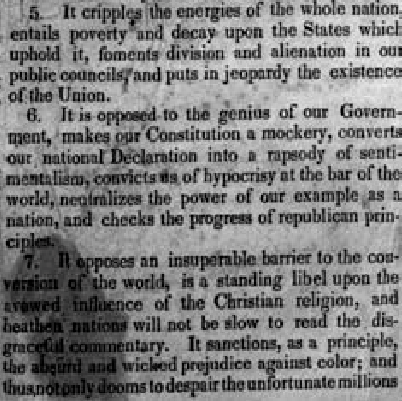
\includegraphics[width=.7\linewidth]{Images/Grayscale.png}
        \caption{Početna crno-bijela slika}
        \label{fig:sub1}
    \end{subfigure}%
    \begin{subfigure}{.5\textwidth}
        \centering
        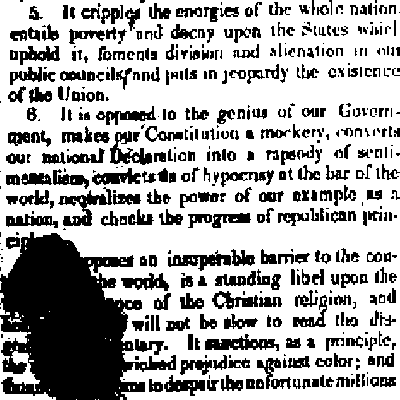
\includegraphics[width=.7\linewidth]{Images/Threshold.png}
        \caption{Slika dobivena binarizacijom fiksnim pragom}
        \label{fig:sub2}
    \end{subfigure}
    \caption{Primjer binarizacije fiksnim pragom}
    \label{fig:threshold}
\end{figure}

\section{Adaptivna binarizacija}
Problemi prikazani u prethodnom postupku rješavaju se primjenom adaptivne binarizacije koja vrijednost sakog pojedinog slikovnog elementa ne određuje samo na osnovu njegove boje, već u obzir uzima i boju okoline.
U nastavku je opisan postupak koji je predložen u \cite{AdaptiveBinarization}.
Prikazani primjeri koriste sliku \ref{fig:sub1} kao početnu.

\subsection{Filtriranje šuma}
Ovisno o stanju dokumenta i načinu digitalizacije istoga moguće je da se na dobivenoj slici pojavljuje šum, kojega je potrebno otkloniti.
Za potrebe opisanoga koristi se niskopropusni Wiener filter \cite{book:Two-Dimensional-Signal-Image-Processing}, koji se temelji na statističkoj procjeni temeljenoj na okruženju svakog pojedinog slikovnog elementa. \cite{AdaptiveBinarization}
Označimo sa $I_s(x, y)$ vrijednost slikovnog elementa početne slike, a sa $I(x, y)$ vrijednost slikovnog elementa filtrirane slike.
Tada se filtrirana slika $I$ može izračunati pomoću formule:
\[I(x, y) = \mu(x, y) + \frac{\sigma(x, y)^2}{(\sigma(x, y)^2 - v^2)}(I_s(x, y) - \mu(x, y))\]
Sa $\mu(x, y)$ označena je aritmetička sredina vrijednosti slikovnih elemenata u okruženju veličine $NxM$, prema formuli:
\[\mu(x, y) = \frac{1}{NM} 
    \displaystyle \sum_{i = x-\frac{N}{2}}^{x+\frac{N}{2}}
    \displaystyle \sum_{j = y-\frac{M}{2}}^{y+\frac{M}{2}}
I_s(i, j)\]
Sa $\sigma^2$ označena je varijanca vrijednosti slikovnih elemenata u okruženju veličine $NxM$, prema formuli:
\[\sigma(x, y)^2 = \frac{1}{NM} 
    \displaystyle \sum_{i = x-\frac{N}{2}}^{x+\frac{N}{2}}
    \displaystyle \sum_{j = y-\frac{M}{2}}^{y+\frac{M}{2}}
(I_s(i, j)^2 - \mu^2)\]
Sa $v^2$ je označena srednja vrijednost svih lokalnih varijanci.
Konačan rezultat filtriranja prikazan je na slici \ref{fig:wiener}.

\begin{figure}[ht!]
    \centering
    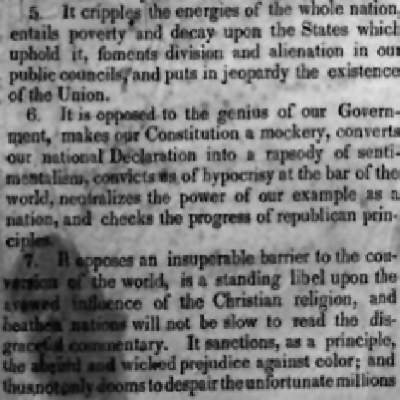
\includegraphics[width=.35\textwidth]{Images/Wiener.png}
    \caption{Slika dobivena binarizacijom fiksnim pragom}
    \label{fig:wiener}
\end{figure}

\subsection{Procjena sadržaja}
\subsection{Procjena pozadine}
\subsection{Binarizacija}
\subsection{Dodatna obrada slike}


\chapter{Prepoznavanje zakrivljenosti slike}

\chapter{Detekcija tablice}
\section{Detekcija vrhova ćelija}
\section{Rekonstrukcija tablice}

\chapter{Primjena na automatskom prepoznavanju rukom pisanih simbola}

\chapter{Zaključak}
Zaključak.


\bibliography{literatura}
\bibliographystyle{fer}

\begin{sazetak}
Sažetak na hrvatskom jeziku.

\kljucnerijeci{Ključne riječi, odvojene zarezima.}
\end{sazetak}

\engtitle{Table Extraction on Scanned Documents}
\begin{abstract}
Abstract.

\keywords{Keywords.}
\end{abstract}

\end{document}
